\subsection{Non-linear initial perturbation}\label{fargo_nonlin}
In order to focus on the one-arm spiral that emerges in the above
simulation, we here analyse a run with only an initial $m=1$
perturbation in the dead zone. Specifically, we set
\begin{align}
  &\Sigma \to \Sigma_0(R) + \delta\Sigma_0(R) + 2\Sigma_1(R)\cos{\phi},\\
  &v_\phi  \to v_{\phi 0}(R) + 2v_{\phi 1}(R)\cos{\phi},
\end{align}
for $R\in[R_{d1},R_{d2}]$, where
\begin{align}
  &\delta\Sigma_0 =
  -\delta^2\times\Sigma_0(R_{d1})\frac{R_{d1}}{R}\sin^3{\left[\frac{2\pi\left(R-R_{d1}\right)}{R_{d2}-R_{d1}}\right]},\\ 
  &\Sigma_1 =
  \delta\times\Sigma_0\sin{\left[\frac{\pi\left(R-R_{d1}\right)}{R_{d2}-R_{d1}}\right]},  
\end{align}
with $\delta = 10^{-3}$, and
\begin{align}
  v_{\phi 1} = -\frac{v_{\phi 0}\delta\Sigma_0}{2\Sigma_1}. 
\end{align}
This perturbs the dead zone structure while conserving total mass and
angular momentum. The $m=1$ perturbation has an associated negative
angular momentum (as observed in the previous simulation) at the
expense of increasing the angular momentum associated with the
background disc. %local exchange for simplicity 
%actually doesn't matter if we set plus or minus
Note that the perturbation to the axisymmetric surface density is
$O(\delta^2)$, whereas that in $m=1$ is $O(\delta)$. Since $Q>1$
everywhere in the disc, there is no risk of axisymmetric gravitational
instability. 

While the above form of initial perturbations is artificial, we find 
the spiral that forms have similar properties (see below) to that found in the
previous simulation, but the above procedure has the 
advantage of producing cleaner results without complications from
higher $m$ modes, and the required simulation time for the one-arm
spiral to emerge is reduced. 

Fig. \ref{2d_angmom_ex} shows the evolution of angular momenta. For
$t\lesssim 15P_0$ there is angular momentum exchange between the
background and the imposed perturbation, but no overall growth takes
place. After $t\gtrsim15P_0$, however, the angular momenta stops 
oscillating and grows monotonically in magnitude.     

\begin{figure}
  % scale=0.41
  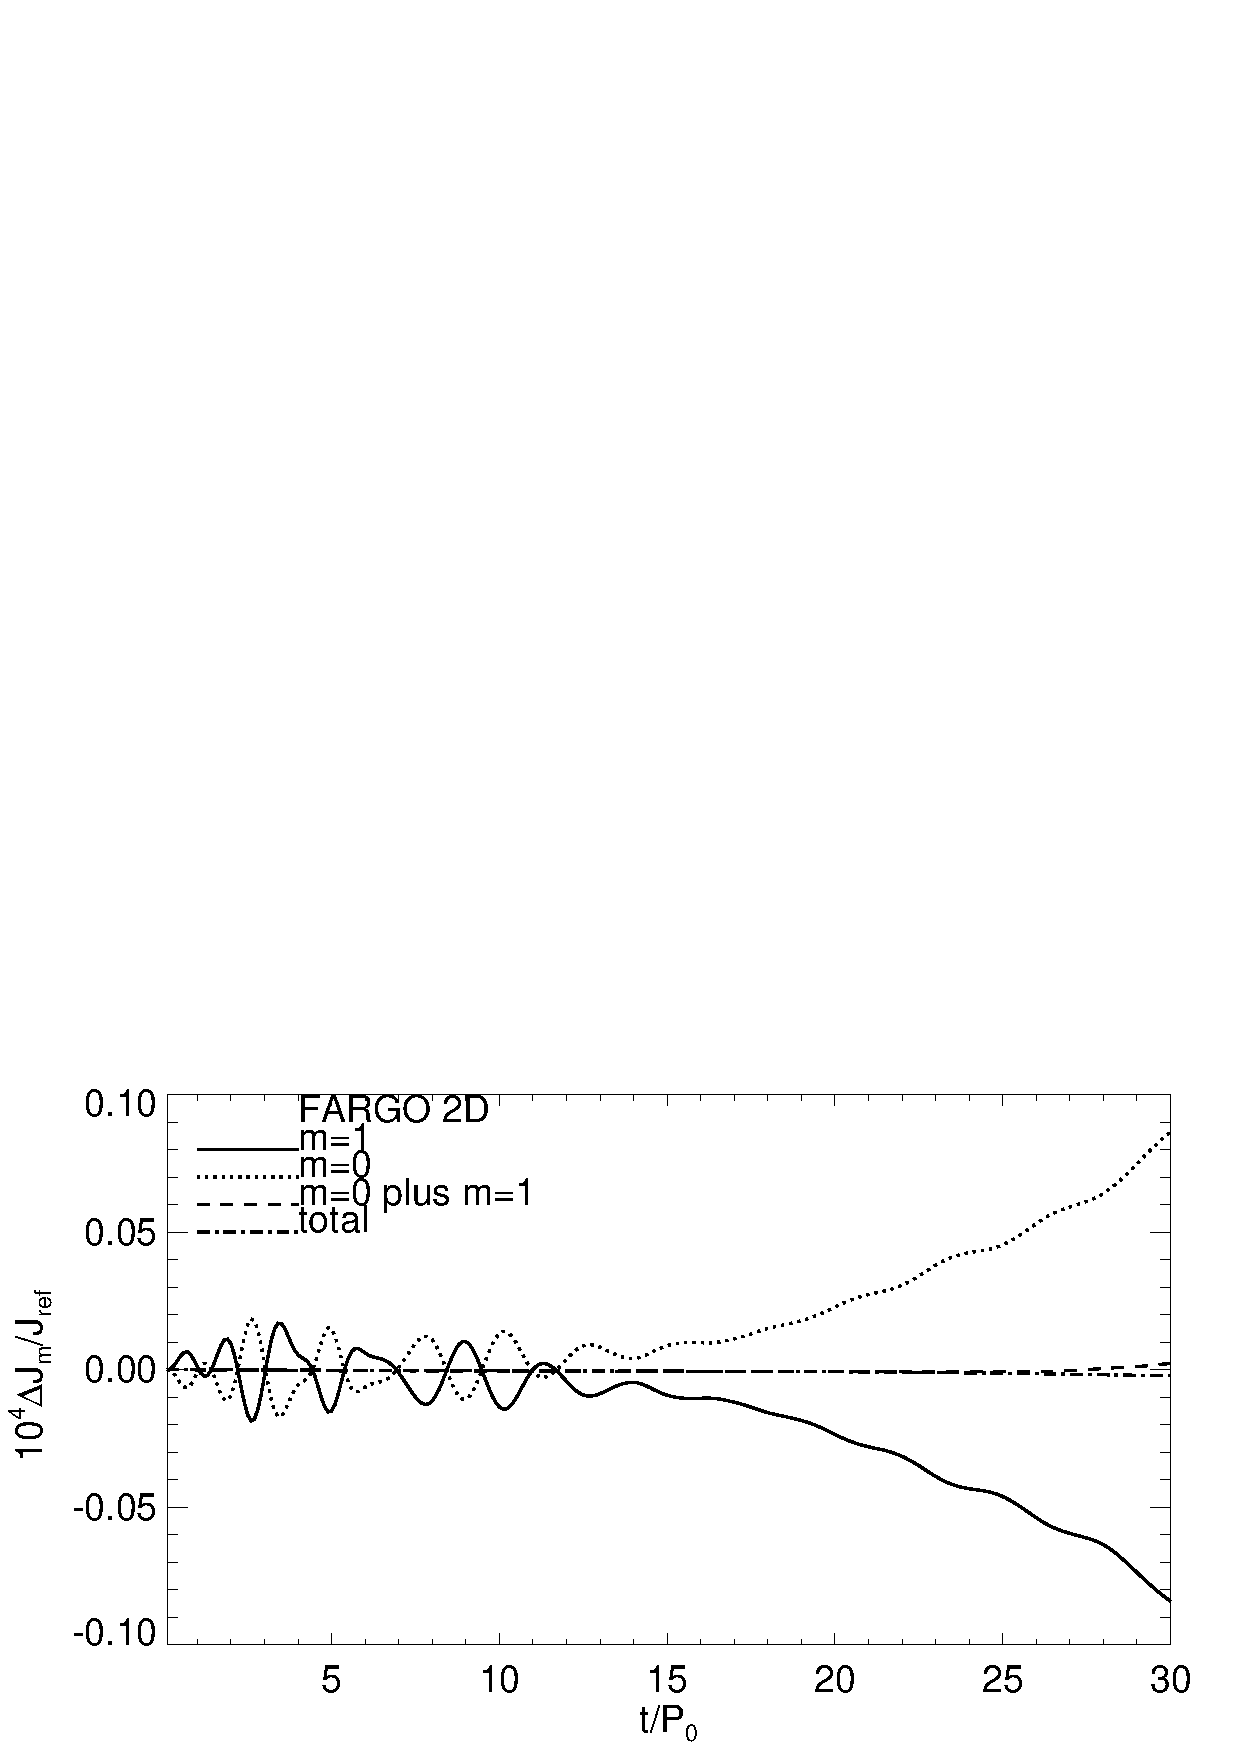
\includegraphics[width=\linewidth]{figures/nonaxi_evol_ang_fargo_ex}
  \caption{Evolution of angular momentum components in the 
    FARGO simulation with the special $m=1$ initial perturbations
    described in \S\ref{fargo_nonlin}. 
    The perturbed angular momentum
    relative to $t=0$ is shown in units of the initial total angular
    momentum $J_\mathrm{ref}=J(t=0)$.\label{2d_angmom_ex}}  
\end{figure}  

Fig. \ref{2d_angmom_ex_evol} show snapshots of the $m=1$
surface density at $t=10P_0$, when angular momenta oscillate; 
$t=15P_0$, when angular momenta stops oscillating; and
$t\in[20,30]P_0$, during the growth phase. 



\begin{figure*}
  % scale=0.41
  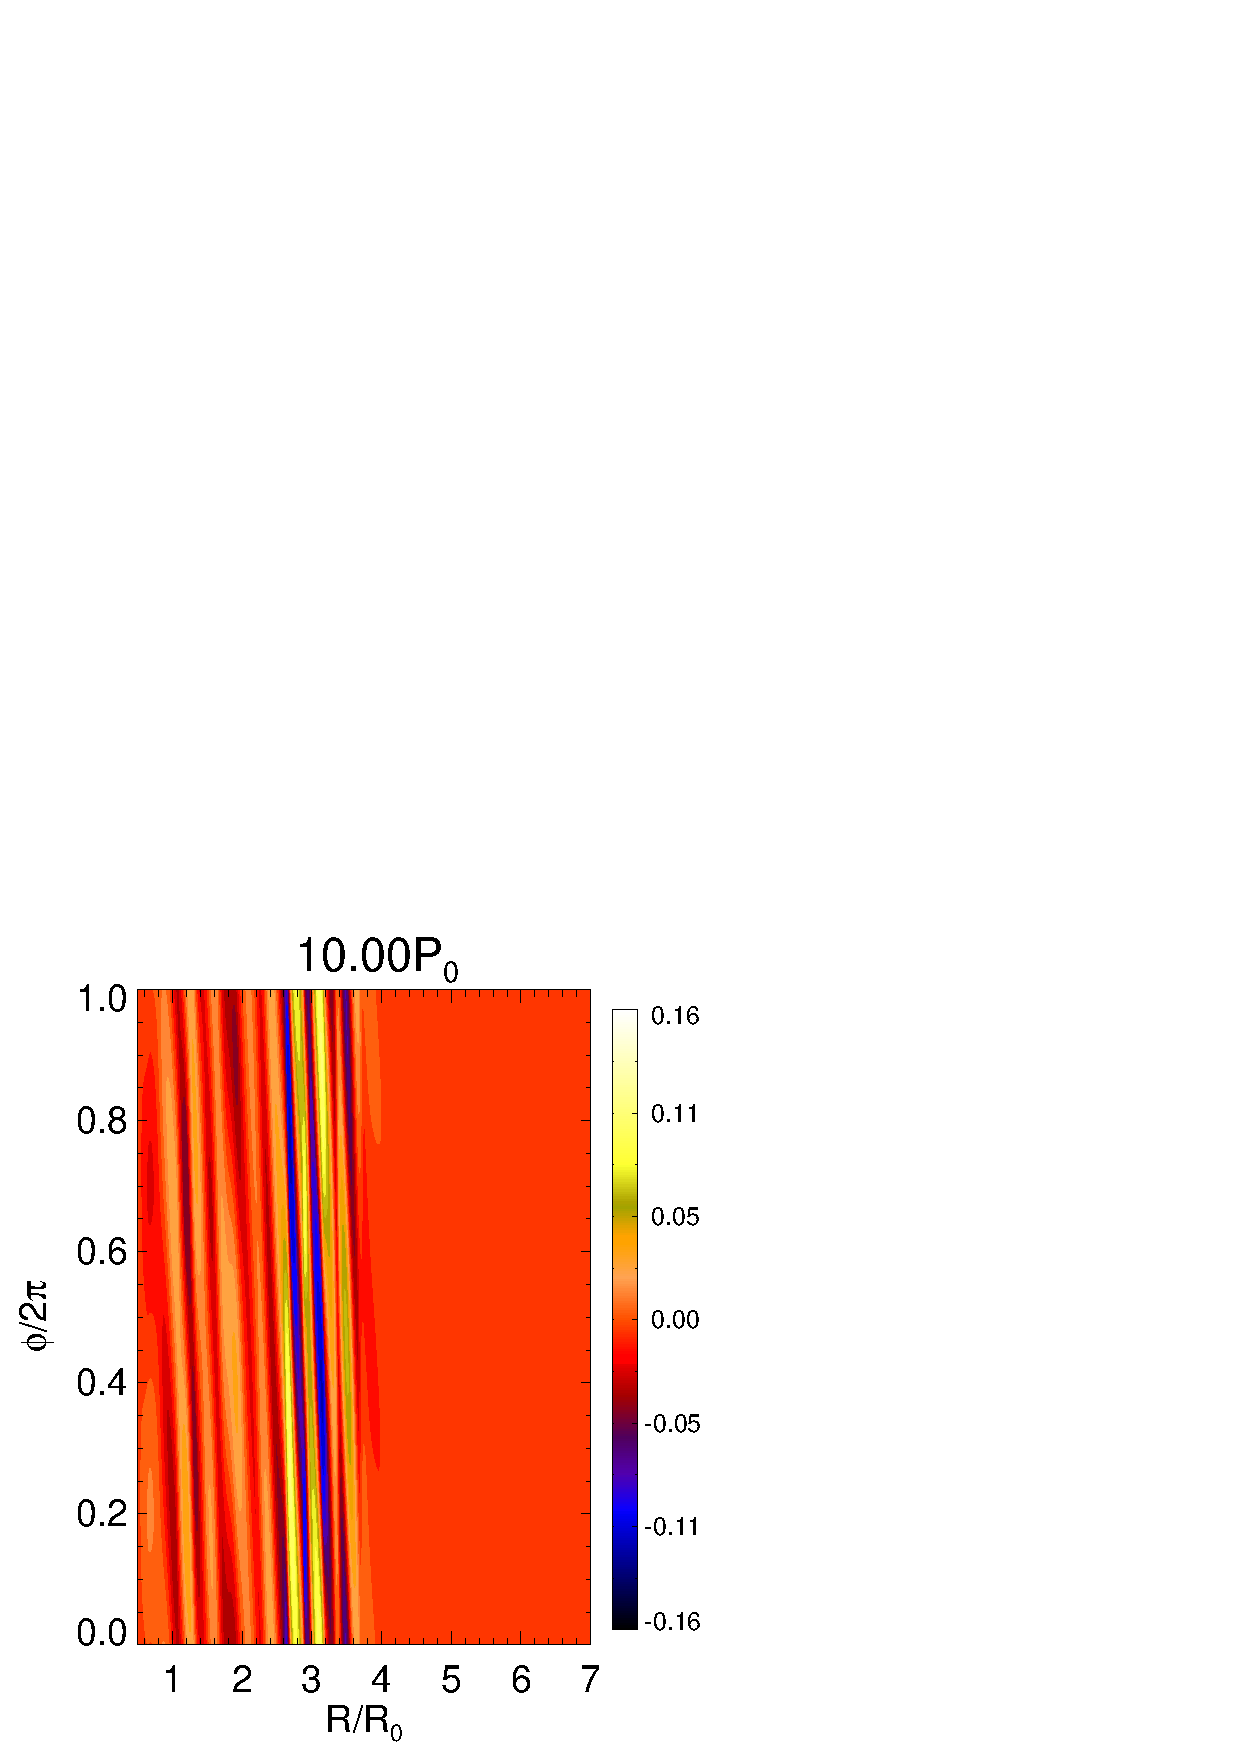
\includegraphics[scale=0.4,clip=true,trim=0cm 0cm 1.73cm
  0cm]{figures/polarxy_fargo_ex_100}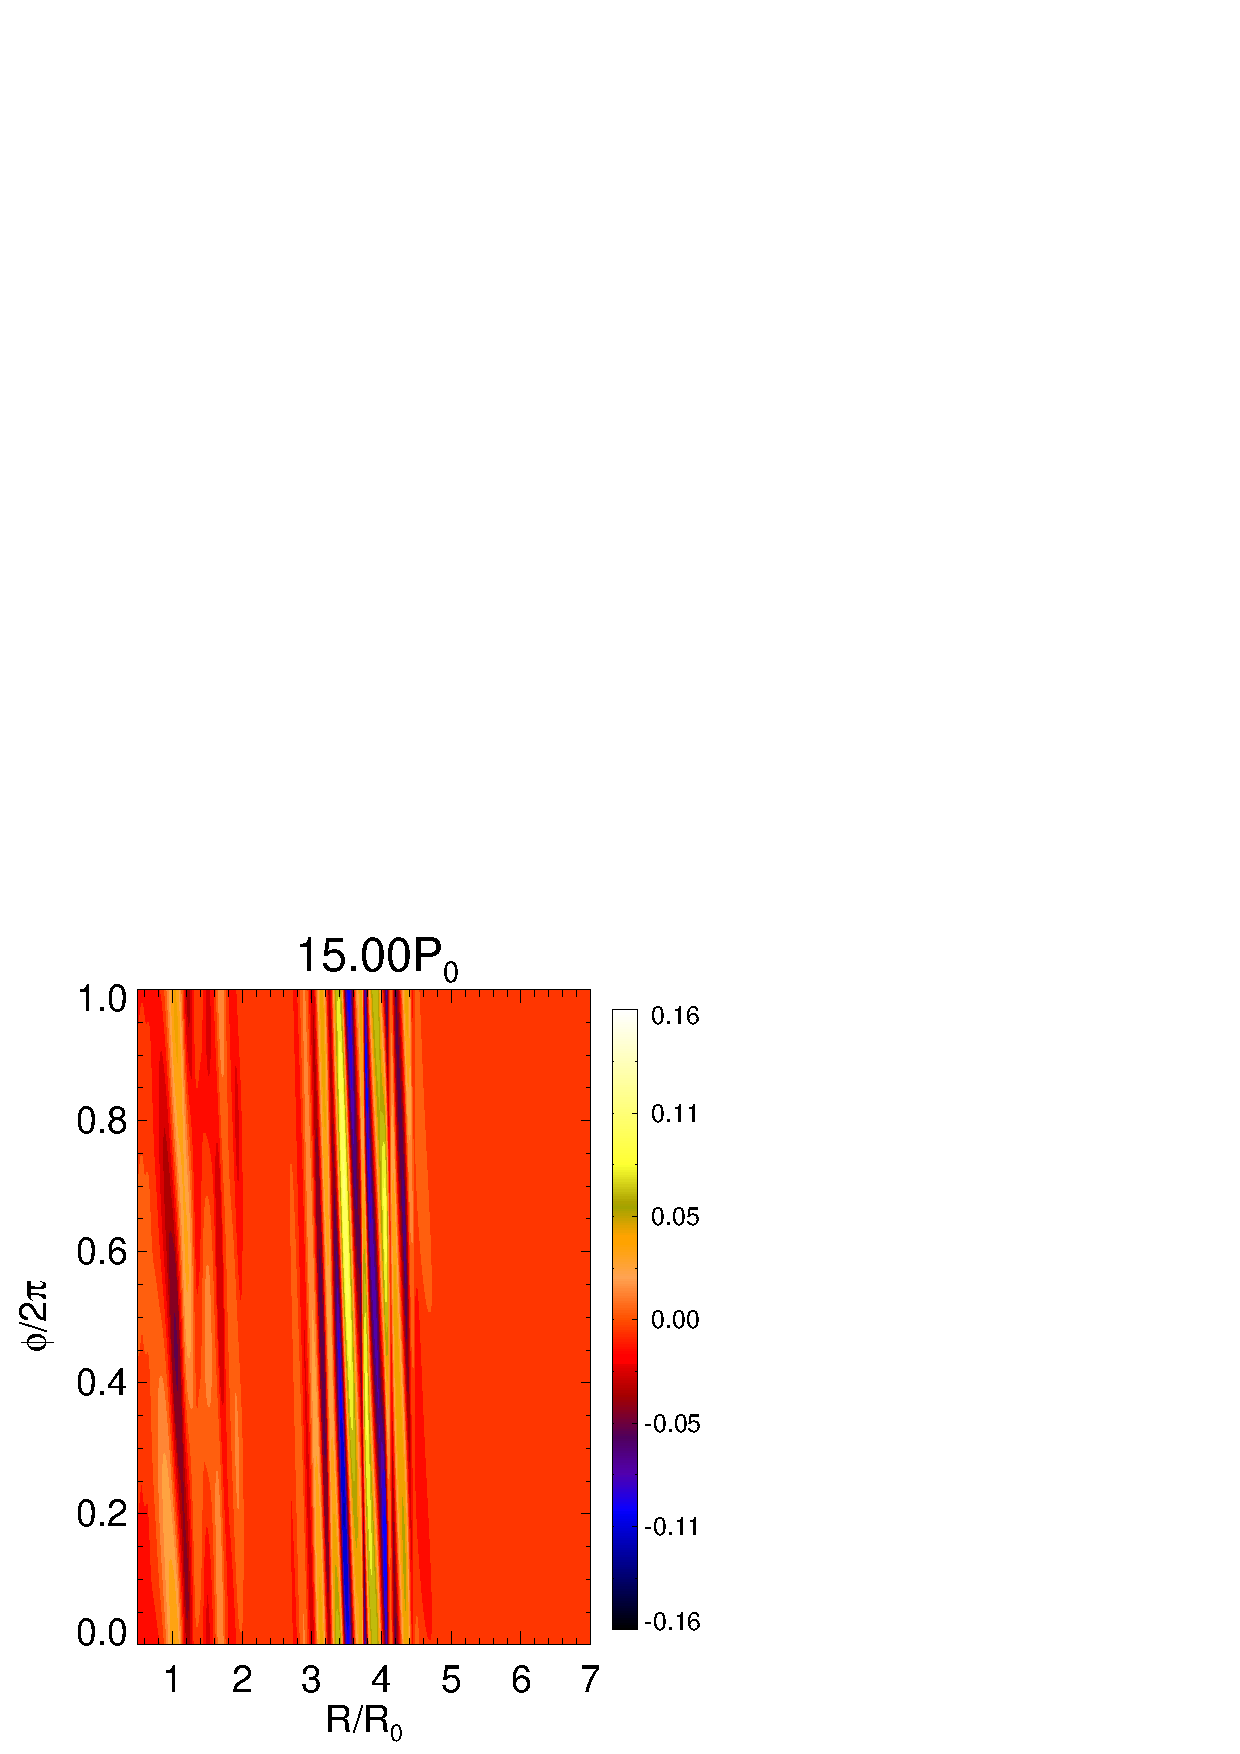
\includegraphics[scale=0.4,clip=true,trim=2.24cm
  0cm 1.73cm 0cm]{figures/polarxy_fargo_ex_150}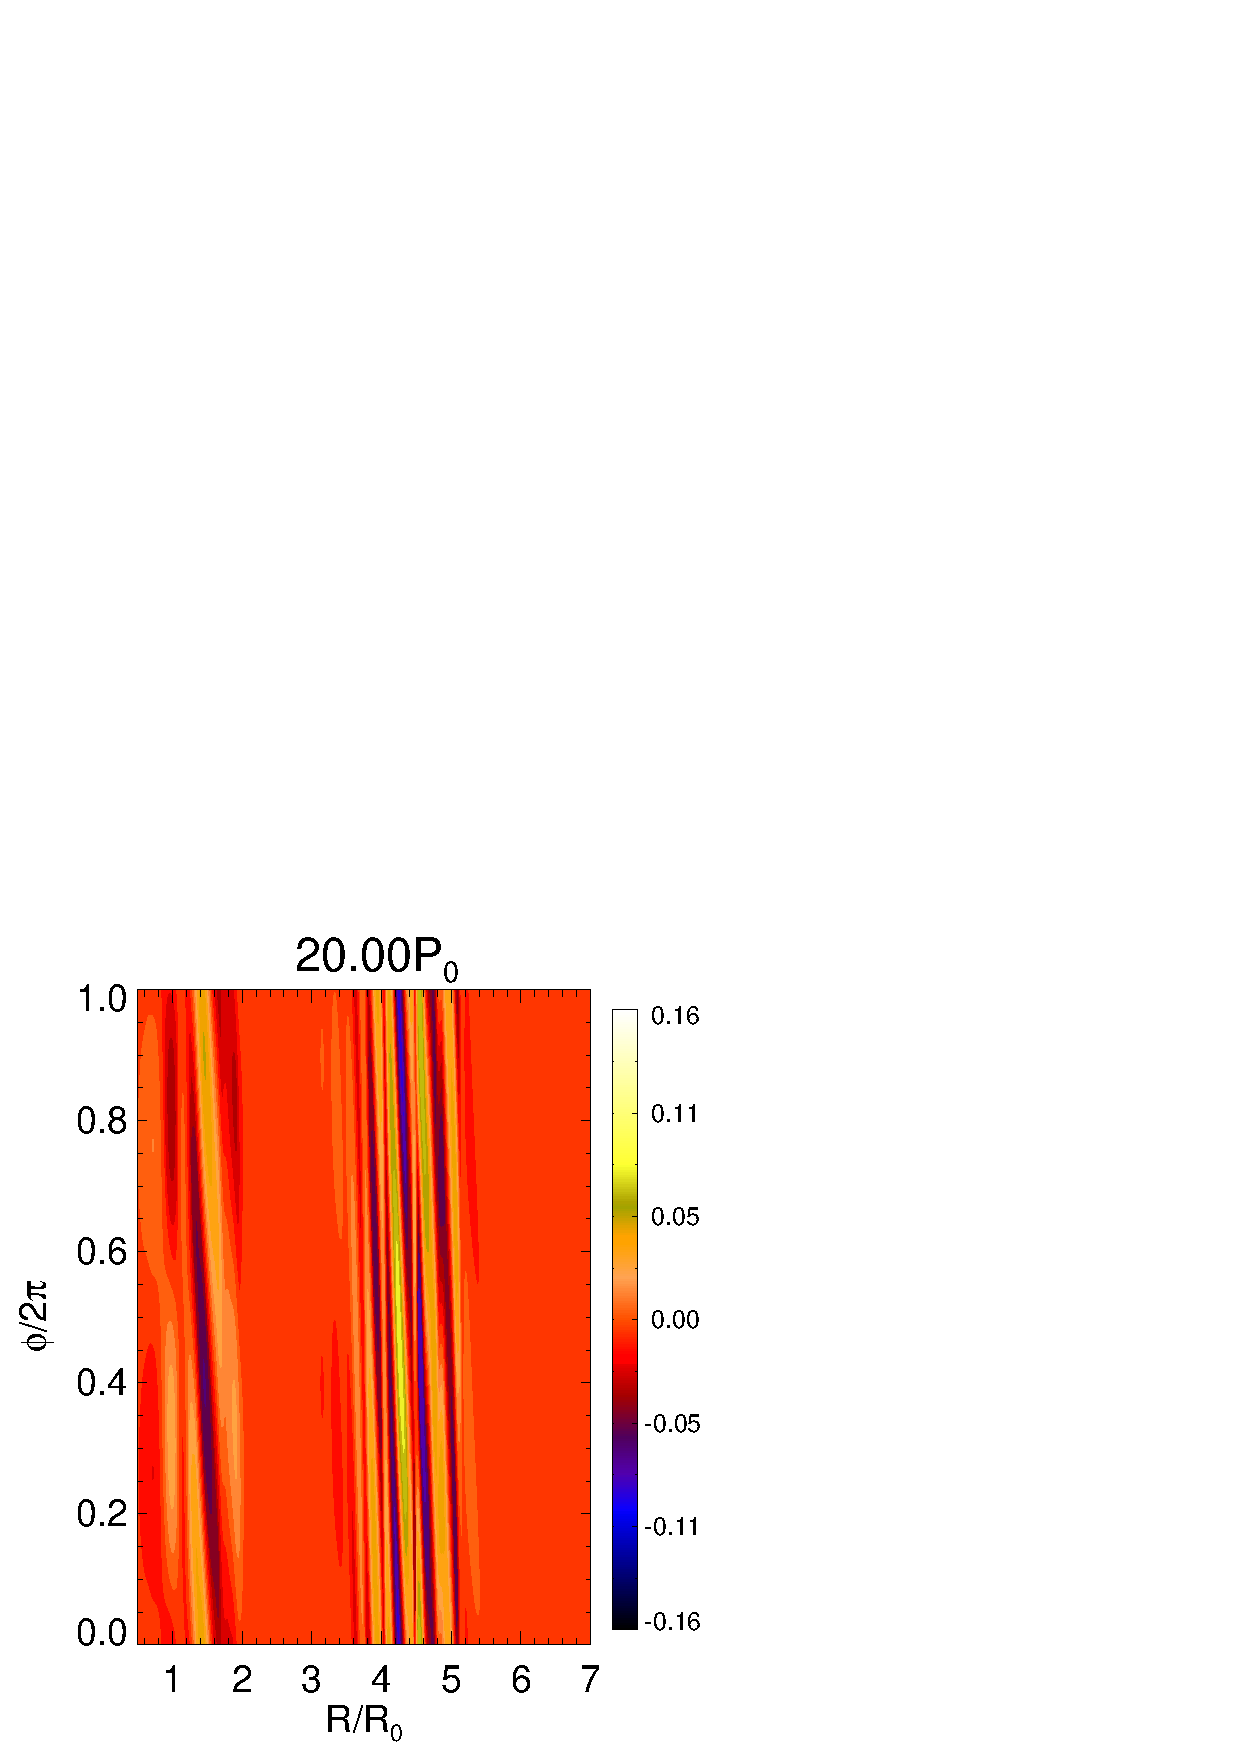
\includegraphics[scale=0.4,clip=true,trim=2.24cm
  0cm 1.73cm 0cm]{figures/polarxy_fargo_ex_200}\includegraphics[scale=0.4,clip=true,trim=2.24cm
  0cm 1.73cm 0cm]{figures/polarxy_fargo_ex_250}\includegraphics[scale=0.4,clip=true,trim=2.24cm
  0cm 0.0cm 0cm]{figures/polarxy_fargo_ex_300}
  \caption{Evolutoin of the $m=1$ surface density in the FARGO
    simulation with the special $m=1$ initial perturbations
    described in \S\ref{fargo_nonlin}. 
    \label{2d_angmom_ex_evol}} 
\end{figure*}  
